\section{Introduction}

The LHC collimation system is a key part of the machine protection system in the LHC. Due to extremely high stored beam and magnetic energy in the LHC \cite{Schmidt:LHCMP}, amounting to some 360MJ of beam energy and 10GJ of stored magnetic energy, it is neccessary to keep close control on the losses experienced by the system. In the LHC this is done by a combination of monitoring the losses within the machine, carefully controlled losses by the collimation system, and a rigorous interlock system designed to dump the beam safely in the event of the development of dangerous behaviour by the circulating beam or a malfunction by safety critical equipment \cite{Schmidt:LHCMP}.

The collimation system in the LHC is a four-stage system, composed primarily of primary (TCP), secondary (TCS), and tertiary (TCT) collimators. These serve to scatter the particle halo, then further scatter and absorb the scattered particles, the schematic of the process shown in Fig.~\ref{fig:colSystemLayout}. Further protection is provided by absorbers (TCLA), collimators at the injection regions (TCLI and TDI) and at the extraction region (TCDQA). In particular the TCTs are placed near the experimental IPs (Interaction Points) to protect the inner triplet magnets (used for final focusing of the beam before collision). In total the collimation system is broken down into two IPs; IR3 for momentum cleaning, in which there are:

\begin{enumerate}
\item{1 primary collimator}
\item{4 secondary collimators}
\item{4 absorbers}
\end{enumerate}

per beam and IR7 for betatron cleaning, which is composed of:

\begin{enumerate}
\item{3 primary collimators}
\item{11 secondary collimators}
\item{5 absorbers}
\end{enumerate}

per beam, with an additional 8 tertiary collimators (2 per experimental IP) per beam. In summary, with the addition to the collimators at the injection and extraction regions each beam is exposed to 44 different moveable collimators per circulation of the machine. The primary and secondary collimators presently all have a jaw material carbon reinforced graphite (conductivity $\sigma_{graphite} = 7 \times 10^{4} S m^{-1} $ for the jaw material). This material was chosen due to the requirement for a robust jaw material (mechanically stable under large thermal shock) from a machine protection point of view, however not optimised from a beam impedance point of view.

\begin{figure}
\begin{center}
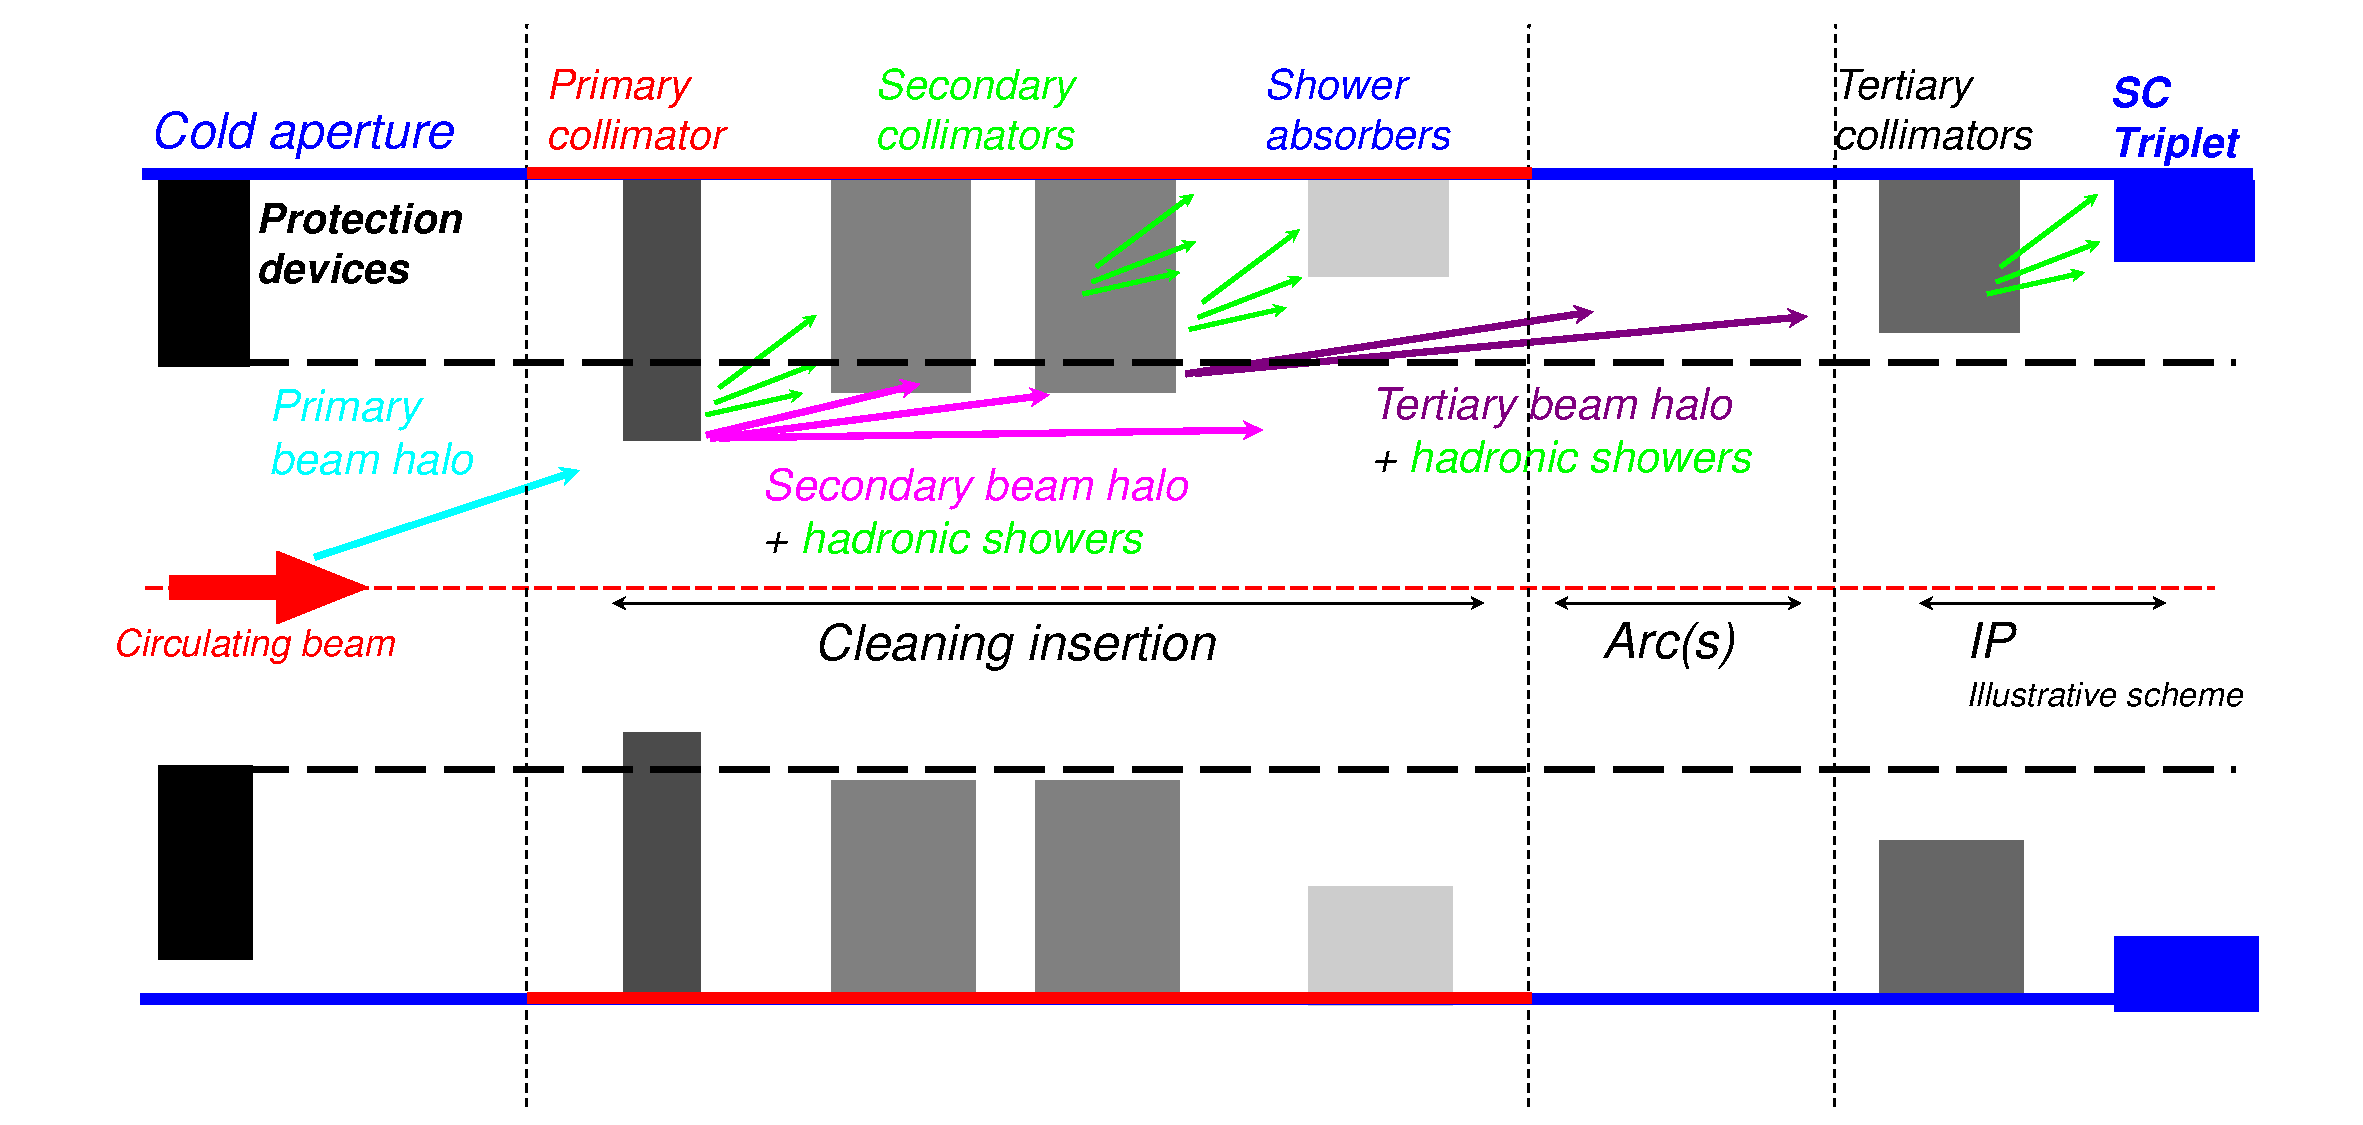
\includegraphics[width=0.9\textwidth]{LHC_Collimation_Upgrades/figures/collimationSchematic.pdf}
\end{center}
\caption{The processes by which the collimation system in the LHC acts to clean the beam and manage losses in a controllable way.}
\label{fig:colSystemLayout}
\end{figure}

The current collimation system has demonstrated to be exceptionally effective at it's job of providing machine protection to the LHC \cite{Zerlauth:MP}, however it has some drawbacks. The very large imaginary component of the transverse impedance gave some worry of being a contributor to instabilities in the LHC, but recent work has shown that there is still some substantial overhead in the stability limit driven by beam coupling impedance. However, interactions with other mechanisms such as beam-beam and electron cloud may produce instabilities at lower intensities \cite{Mounet:PhDThesis}. 

\begin{figure}
\begin{center}
\subfigure[]{
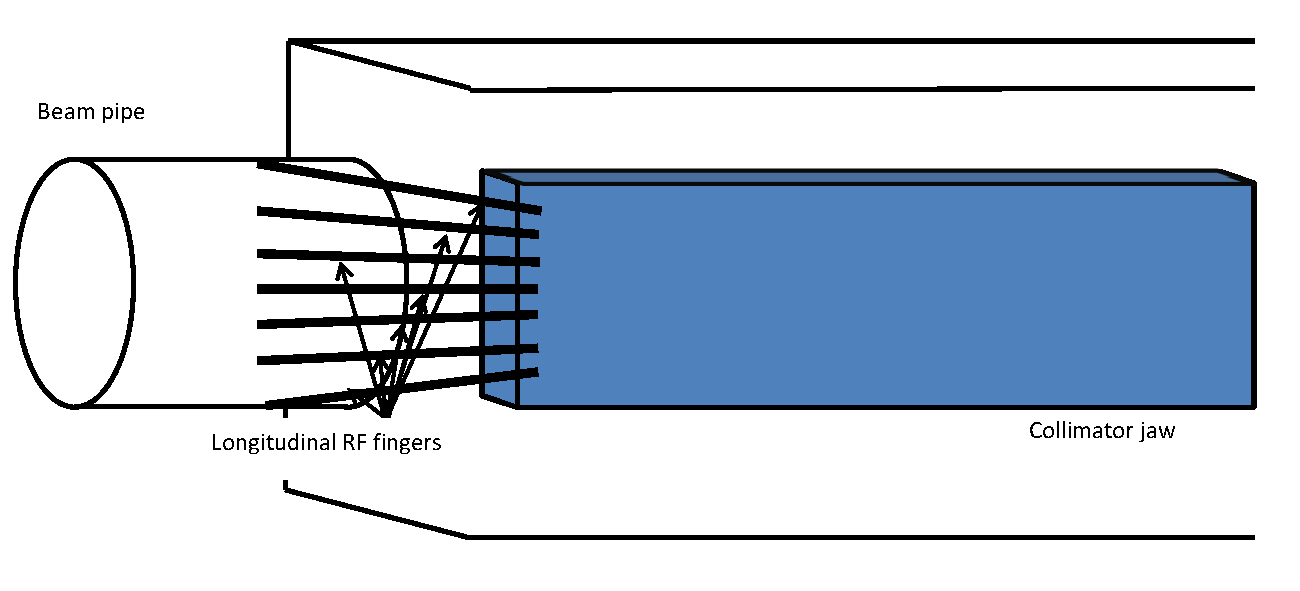
\includegraphics[width=0.9\textwidth]{LHC_Collimation_Upgrades/figures/longitudinalRFFingers.pdf}
\label{fig:phase-1-col-longitudinal-rf}
}

\subfigure[]{
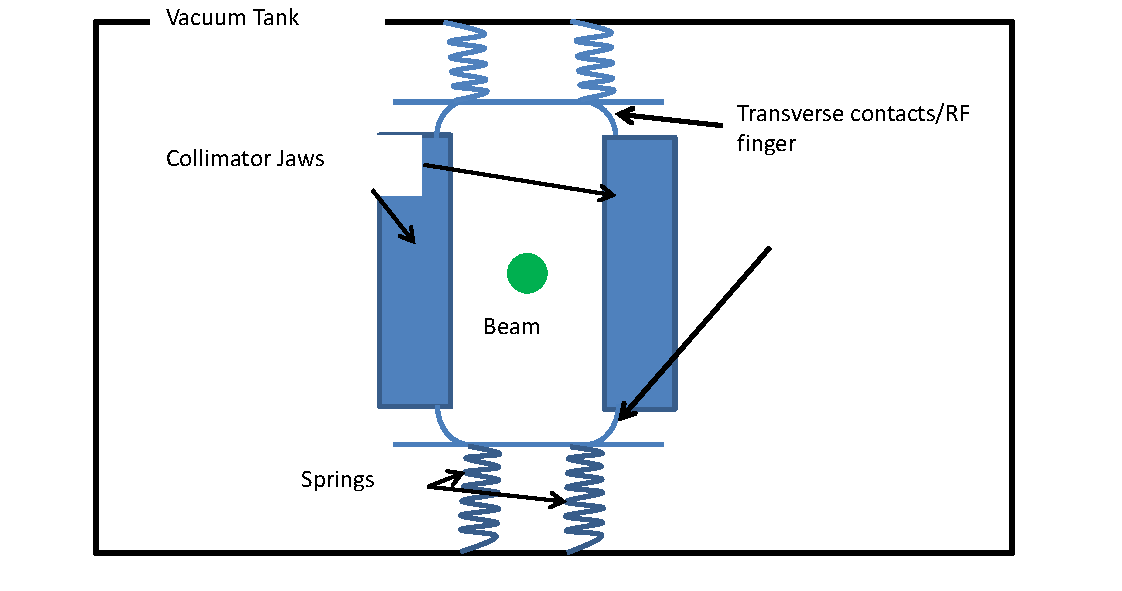
\includegraphics[width=0.9\textwidth]{LHC_Collimation_Upgrades/figures/transverseRFFingers.pdf}
\label{fig:phase-1-col-sliding-contacts}
}
\end{center}
\caption{Different components of impedance reduction measures in the phase 1 collimator design. \ref{fig:phase-1-col-longitudinal-rf} shows the longitudinal RF fingers, ensuring a good conducting path for the beam image currents, and \ref{fig:phase-1-col-sliding-contacts} shows the sliding RF contacts on the collimators jaw. These are intended to minimise the volume seen by the beam, thus minimising any cavity modes that may be excited by the beam at very high frequencies where the beam power spectrum is very small.}
\label{fig:phase-1-rf}
\end{figure}

The phase 1 collimator (those presently (as of 2012) in place in the LHC) design has a number of design features that are designed to reduce the beam coupling impedance of each device. Although the resistive wall contribution to the beam coupling impedance, due to the poorly conducting jaw material, is significant, the use of longitudinal RF fingers in the transition between the beam pipe to the collimator jaws and of a system of sliding contact fingers isolates the beam from seeing the collimator vacuum tank (see Fig~\ref{fig:phase-1-rf} for more details). These function well as impedance reduction techniques, however have some limitations from a mechanical point of view. In particular, the sliding contacts have been suspected to be a significant producer of dust in the LHC due to the moving physical contact during collimator alignment and some collimators were suspected (and a number observed) with RF fingers with broken contact. 

Due to these factors (high transverse impedance due to the resistive wall impedance, problems of dust due to sliding contacts and possible RF fingers not touching) a phase 2 upgrade of the LHC collimation system has been proposed. This entails two components;

\begin{enumerate}
\item{The supplementation of the current secondary collimators (the prime contributor to the large transverse impedance) by a phase 2 design using a good conducting material as the jaw material. There will be some loss of mechnical robustness but it is thought that this will not be detrimental to the requirements of machine protection with a suitable choice of material.}
\item{Replacing the existing sliding RF contacts with a contactless RF system (shown in Fig.~\ref{fig:phase-2-rf-system}). This is designed to suppress the problem of dust caused by the sliding RF contacts in the phase 1 system by removing the moving physical contacts in addition to being more mechanically robust. This increases the volume of the cavity visible to the particle beam, decreasing the frequency of the lowest cavity modes. To counteract these new resonances, ferrite is placed in the cavity to decrease the resulting Q of the resonances.}
\end{enumerate}

\begin{figure}
\begin{center}
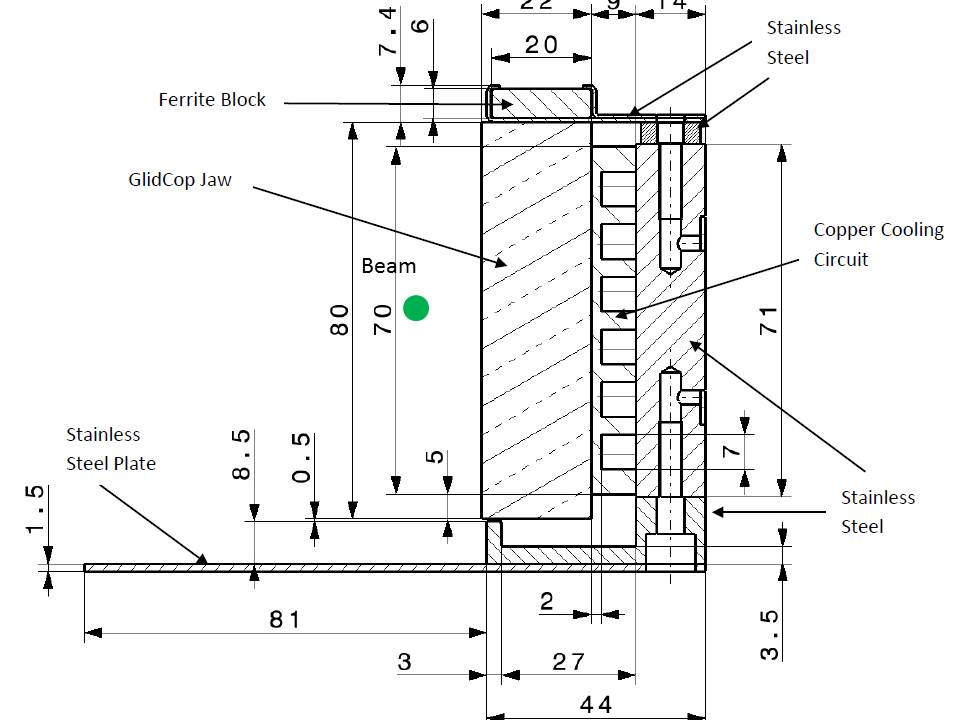
\includegraphics[width=0.7\textwidth]{LHC_Collimation_Upgrades/figures/cu-geo.jpg}
\end{center}
\caption{The RF system for use in the phase 2 collimation system. The sliding RF contacts of the phase 1 design are replaced with a ferrite damping system. The RF contacts are removed, allowing the beam to see the entire RF cavity, causing resonances at lower frequencies. The Q of these resonances are decreased by the use of ferrite damping tiles (see Sec.~\ref{sec:damping_materials}). the location of the beam is shown in green.}
\label{fig:phase-2-rf-system}
\end{figure}

In this chapter shall be presented an comparison of the different jaw materials proposed for use in the phase 2 secondary collimators. In particular a combination of jaw materials aimed at combining extremely robust materials with highly conductive metals, and the results of full 3D simulations of a TCTP collimator - a tertiary collimator for use in the LHC - which incorporates the ferrite damping system, is compared to the sliding contacts of the phase 1 RF system. 



%
% Introduction to the new collimator design - Old collimator design, problems with sliding rails, new design, new material possibilities
% Material Evaluation - Comparison of CST simulations
% Whole collimator simulations of phase 2 secondary - Transverse and longitudinal modes with ferrite - compared to that from phase 1
% Sims in CST PS, GdFidl and HFSS
% Heating calculations also
%
%
%
%
%


